\documentclass[conference]{IEEEtran}

\usepackage{graphicx}
\usepackage{booktabs}
\usepackage{amsmath}
\usepackage{amssymb}
\usepackage{hyperref}
\usepackage{float}
\usepackage{algorithm}
\usepackage{algorithmic}

\title{GPU Accelerated Approximate Bayesian Computation: \\
A Dual Workload Sequential Baseline}

\author{\IEEEauthorblockN{Tejal, Dhyan, Vinay, Arya}
\IEEEauthorblockA{CS F422 Parallel Computing, BITS Goa\\
f20240558@goa.bits-pilani.ac.in}}

\begin{document}

\maketitle

\begin{abstract}
Approximate Bayesian Computation (ABC) enables parameter inference when a
likelihood function is unavailable, but its repeated forward simulations can be
computationally very expensive. We wrote a single threaded C++ ABC rejection
sampler and checked it on two models that do not cost the same to run. The
Gaussian case has a known posterior so we can tell if the sampler is right. The
discrete time stochastic Susceptible--Infected--Recovered (SIR) model is slower
and some particles finish earlier than others if we stop when $I=0$. We also
run SIR for a fixed $T$. Particle counts are $10^4$, $10^5$, and $10^6$. The
timings here are what we will compare against once the CUDA version exists.
\end{abstract}

\begin{IEEEkeywords}
Approximate Bayesian Computation, simulation-based inference, CUDA, parallel
computing, SIR epidemic model, performance baseline.
\end{IEEEkeywords}

\section{Introduction}

Approximate Bayesian Computation (ABC) is used when the likelihood is hard or
impossible to write down. Instead of evaluating the likelihood, ABC draws
parameters from a prior, runs a simulator, and keeps the parameters whose
simulated output is close enough to the observed data~\cite{beaumont2002approximate}.
It shows up a lot in genetics, epidemiology, and ecology, where you have a
simulator but not a closed form likelihood~\cite{sisson2018handbook}.

Particles do not depend on each other, so the loop over $N$ can be split across
GPU threads. Kulkarni et al.\ ran batched ABC for epidemiology models on
accelerators~\cite{kulkarni2022hardware}. ABCpy looked at parallel ABC from an
HPC angle, including load imbalance when simulations do not all cost the
same~\cite{dutta2021abcpy}.

A CUDA number is not useful unless the sequential code is right and the
simulator is heavy enough that launch overhead is not the whole story. So this
milestone is a single threaded C++ rejection sampler on:
\begin{itemize}
    \item a Gaussian model with a known posterior;
    \item a discrete time stochastic SIR model, stopping early when $I=0$ or
          always running $T$ steps.
\end{itemize}

Milestone 1 is the CPU code and the numbers in the tables. CUDA is next.

The CPU RNG is xoshiro256** with Box--Muller. On the GPU we will probably use
cuRAND or Philox, so the accepted lists will not be the same draws. Mean,
variance, and acceptance rate are what we will match.

\section{Related Work}

Beaumont et al.~\cite{beaumont2002approximate} introduced ABC for population
genetics. Sisson et al.~\cite{sisson2018handbook} cover the usual variants
and how people pick the tolerance.

Kulkarni et al.~\cite{kulkarni2022hardware} parallelized the sample, simulate,
and distance stages of batched ABC on accelerators. We are following that
setup in CUDA later. ABCpy~\cite{dutta2021abcpy} used MPI and noted that some
particles take longer than others.

In a stochastic SIR run, some epidemics die out early and take fewer steps.
On a GPU that shows up as thread divergence. We timed both early exit and
fixed $T$ on the CPU so those two effects are not mixed together later.

\section{Problem Definition}

\subsection{ABC Rejection Sampling}

We have observed data $y_{\mathrm{obs}}$, a prior $\pi(\theta)$, a simulator
$f(\theta) \to y_{\mathrm{sim}}$, summaries $S(\cdot)$, a distance
$d(\cdot, \cdot)$, and a tolerance $\varepsilon > 0$. Each particle does:
\begin{enumerate}
    \item Sample $\theta^* \sim \pi(\theta)$.
    \item Simulate $y_{\mathrm{sim}} = f(\theta^*)$.
    \item Compute $s_{\mathrm{sim}} = S(y_{\mathrm{sim}})$.
    \item Accept $\theta^*$ if
          $d(s_{\mathrm{sim}}, s_{\mathrm{obs}}) \leq \varepsilon$.
\end{enumerate}
Accepted $\theta$ values come from
$\pi(\theta \mid d(S(f(\theta)), s_{\mathrm{obs}}) \leq \varepsilon)$.
Sisson et al.\ note that this target approaches the true posterior when
$\varepsilon$ is taken to zero~\cite{sisson2018handbook}. With a nonzero
$\varepsilon$ we only expect the mean and variance to land near the exact
values.

\subsection{Workload 1: Gaussian Inference Model}

For Gaussian ABC we can compare against a closed form posterior.

\begin{itemize}
    \item \textbf{Prior:} $\theta \sim \mathcal{N}(0, 1)$.
    \item \textbf{Simulator:} $y_{\mathrm{sim}} \sim \mathcal{N}(\theta, 1)$.
    \item \textbf{Observed value:} $y_{\mathrm{obs}} = 1.0$.
    \item \textbf{Summary statistic:} $S(y) = y$.
    \item \textbf{Distance:}
          $d = |y_{\mathrm{sim}} - y_{\mathrm{obs}}|$.
    \item \textbf{Tolerance:} $\varepsilon = 0.1$.
\end{itemize}

At zero tolerance the exact posterior is
\begin{equation}
    \theta \mid y_{\mathrm{obs}} = 1 \sim
    \mathcal{N}\!\left(\frac{1}{2},\; \frac{1}{2}\right).
    \label{eq:gaussian_posterior}
\end{equation}

Each particle is two random draws and one comparison. Table~\ref{tab:gaussian_epsilon}
is the same model at $N=10^5$ for a few $\varepsilon$ values.

\subsection{Workload 2: Stochastic SIR Epidemic Model}

SIR does more work per particle. If the epidemic dies out, early exit also
makes some particles shorter than others.

\subsubsection{Model Parameters}

\begin{itemize}
    \item \textbf{Parameters:} infection rate $\beta$ and recovery rate $\gamma$.
    \item \textbf{Priors:} $\beta \sim \mathrm{Uniform}(0.1, 1.0)$,\;
          $\gamma \sim \mathrm{Uniform}(0.01, 0.5)$.
    \item \textbf{Population:} $N_{\mathrm{pop}} = 1000$, with
          $S_0 = 990$, $I_0 = 10$, $R_0 = 0$.
\end{itemize}

\subsubsection{Discrete-Time Stochastic Simulator}

At each time step $t$:
\begin{align}
    \Delta I_t &\sim \mathrm{Binomial}\!\left(S_t,\;
                 1 - \exp\!\left(-\frac{\beta\, I_t}{N_{\mathrm{pop}}}\right)
                 \right), \label{eq:sir_infections} \\
    \Delta R_t &\sim \mathrm{Binomial}(I_t,\; \gamma),
                 \label{eq:sir_recoveries}
\end{align}
then
\begin{align}
    S_{t+1} &= S_t - \Delta I_t, \quad
    I_{t+1} = I_t + \Delta I_t - \Delta R_t, \quad
    R_{t+1} = R_t + \Delta R_t.
\end{align}

\subsubsection{Two Simulation Modes}

Both modes use the same $\varepsilon$, the same $\sigma_k$, and the same
observed summaries:
\begin{enumerate}
    \item \textbf{Early exit:} stop when $I_t = 0$. Cheap particles finish
          early.
    \item \textbf{Fixed horizon:} always run $T = 160$ steps.
\end{enumerate}
Fixed $T$ keeps the step count the same. Early exit does not. Having both
on CPU means a later GPU timing is not stuck with one of those mixed in.

\subsubsection{Summary Statistics and Distance}

\begin{equation}
    s = \bigl(\text{peak infected count},\;
         \text{time of peak},\;
         \text{final recovered count}\bigr).
\end{equation}
Distance is Euclidean after normalizing each component:
\begin{equation}
    d(s_{\mathrm{sim}}, s_{\mathrm{obs}}) =
    \sqrt{\sum_{k=1}^{3}
      \left(\frac{s_{\mathrm{sim},k} - s_{\mathrm{obs},k}}
                 {\sigma_k}\right)^{\!2}},
    \label{eq:sir_distance}
\end{equation}
where $\sigma_k$ comes from a pilot run and is then kept fixed.

\subsubsection{How we fix SIR settings}

\begin{enumerate}
    \item Simulate one observed trajectory from
          $(\beta, \gamma) = (0.4, 0.1)$ with a fixed seed and save
          $s_{\mathrm{obs}}$.
    \item Run a few thousand draws from the prior, get $\sigma_k$ from those
          summaries.
    \item Set $\varepsilon$ to a quantile of the pilot distances so acceptance
          is about 1--5\%.
    \item Save $s_{\mathrm{obs}}$, $\sigma_k$, and $\varepsilon$. Later CPU
          and GPU runs just read those files.
\end{enumerate}
$\varepsilon$ is left at the pilot quantile for the runs in the tables.

\subsubsection{What counts as correct for SIR}

$(\beta, \gamma)$ is not well identified from three summaries, and there is no
closed form posterior. We look at whether the samples sit nearer $(0.4, 0.1)$
than the prior, and we report mean and spread.

\subsection{Metrics}

For both workloads we report runtime, throughput (particles per second),
number accepted, acceptance rate, and posterior summaries (mean and variance
for Gaussian; means and spread for $\beta$ and $\gamma$ in SIR).

For SIR we also report steps per particle (mean, std, histogram), updates per
second, and early exit vs fixed $T$ at the same $N$.

\section{Sequential Implementation}

\subsection{Architecture}

Models and the sampler are separate. Each model is a struct with
\texttt{sample\_prior}, \texttt{simulate}, \texttt{distance}, and
\texttt{observed\_stats}. Kernels cannot use virtuals or most of the STL, so
the CPU side is already written that way.

Accepted parameters are stored as one array per parameter, which is the layout
we will want for coalesced loads later.

\subsection{ABC Rejection Sampling Algorithm}

Algorithm~\ref{alg:abc} is what both workloads run.

\begin{algorithm}[H]
\caption{Sequential ABC rejection sampling.}
\label{alg:abc}
\begin{algorithmic}[1]
\REQUIRE Model $\mathcal{M}$, particle count $N$, tolerance $\varepsilon$,
         random seed
\ENSURE Accepted parameter samples, summary metrics
\STATE Initialize RNG with seed
\STATE $s_{\mathrm{obs}} \leftarrow \mathcal{M}.\texttt{observed\_stats}()$
\STATE accepted $\leftarrow$ empty list
\STATE Start timer
\FOR{$i = 1$ \TO $N$}
    \STATE $\theta_i \leftarrow \mathcal{M}.\texttt{sample\_prior}(\text{rng})$
    \STATE $s_i \leftarrow \mathcal{M}.\texttt{simulate}(\theta_i, \text{rng})$
    \STATE $d_i \leftarrow \mathcal{M}.\texttt{distance}(s_i, s_{\mathrm{obs}})$
    \IF{$d_i \leq \varepsilon$}
        \STATE Append $\theta_i$ to accepted
    \ENDIF
\ENDFOR
\STATE Stop timer
\STATE Compute and write summary statistics
\end{algorithmic}
\end{algorithm}

\subsection{Implementation Details}

The code is C++17, compiled \texttt{-O2}. RNG is xoshiro256** seeded with
SplitMix64. Normals are Box--Muller. Binomials use geometric waiting times.
We store accepted parameters by column and record how many SIR steps each
particle ran. Command line flags cover model, $N$, $\varepsilon$, seed, and
SIR early exit. Timing runs start at seed $42$; extra reps use $43$, $44$,
and so on. This milestone is single threaded (no CUDA or OpenMP).

Compiler: Apple Clang 17, \texttt{-O2 -std=c++17}, macOS arm64. All timings
are on that machine, one thread.

\section{Experimental Setup}

\subsection{Configuration}

\begin{table}[H]
\caption{Common experiment configuration.}
\label{tab:config}
\centering
\begin{tabular}{ll}
\toprule
Parameter & Value \\
\midrule
Particle counts & $10^4$, $10^5$, $10^6$ \\
Execution model & Single-threaded CPU \\
Random seed & 42 \\
\midrule
\multicolumn{2}{c}{\emph{Gaussian model}} \\
\midrule
Observed value $y_{\mathrm{obs}}$ & $1.0$ \\
Tolerance $\varepsilon$ & $0.1$ \\
\midrule
\multicolumn{2}{c}{\emph{SIR model}} \\
\midrule
Population $N_{\mathrm{pop}}$ & $1000$ \\
Initial infected $I_0$ & $10$ \\
Time steps $T$ & $160$ \\
True parameters & $\beta = 0.4$, $\gamma = 0.1$ \\
Tolerance $\varepsilon$ & $0.382$ (2\% pilot quantile) \\
SIR modes & Early-exit and fixed-$T$ \\
\bottomrule
\end{tabular}
\end{table}

\subsection{Frozen SIR Calibration}

$\sigma_k$ and $\varepsilon$ come from a pilot of a few thousand simulations.
$\varepsilon$ is a quantile of those distances (we wanted about 1--5\%
accepted), not something we tweaked by hand. $s_{\mathrm{obs}}$, $\sigma_k$,
and $\varepsilon$ are saved in the repo and reused as is.

\section{Correctness Validation}

\subsection{Gaussian Model}

Eq.~\ref{eq:gaussian_posterior} is the ground truth. With $\varepsilon = 0.1$
the ABC mean and variance should sit near $0.5$.

\begin{table}[H]
\caption{Gaussian model: posterior validation ($N = 10^6$).}
\label{tab:gaussian_validation}
\centering
\begin{tabular}{lcc}
\toprule
Method & Mean & Variance \\
\midrule
Analytical posterior & $0.500$ & $0.500$ \\
Sequential ABC & $0.501$ & $0.501$ \\
\bottomrule
\end{tabular}
\end{table}

\begin{figure}[H]
\centering
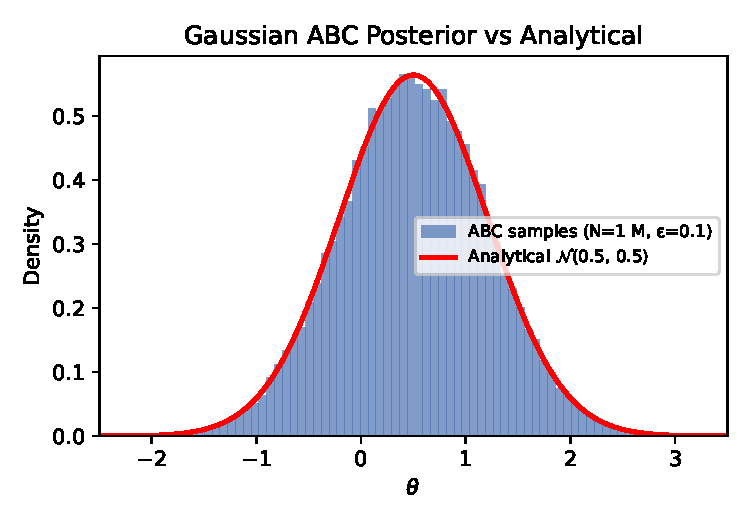
\includegraphics[width=0.96\columnwidth]{../figures/gaussian_posterior.pdf}
\caption{Gaussian ABC posterior vs.\ analytical posterior ($N=10^6$, $\varepsilon=0.1$).}
\label{fig:gaussian_posterior}
\end{figure}

\subsubsection{Approximation Quality vs.\ Tolerance}

\begin{table}[H]
\caption{Gaussian posterior vs.\ tolerance ($N = 10^5$).}
\label{tab:gaussian_epsilon}
\centering
\begin{tabular}{cccc}
\toprule
$\varepsilon$ & Mean & Variance & Acceptance rate \\
\midrule
$1.0$ & $0.420$ & $0.570$ & $42.2\%$ \\
$0.5$ & $0.477$ & $0.518$ & $21.8\%$ \\
$0.1$ & $0.489$ & $0.504$ & $4.4\%$ \\
$0.05$ & $0.480$ & $0.496$ & $2.2\%$ \\
Analytical & $0.500$ & $0.500$ & --- \\
\bottomrule
\end{tabular}
\end{table}

Smaller $\varepsilon$ in Table~\ref{tab:gaussian_epsilon} sits closer to
$N(0.5,0.5)$, with a lower acceptance rate.

\subsection{SIR Model}

SIR has no closed form posterior. We check that the ABC samples move from the
prior toward $(0.4, 0.1)$. With only three summaries we do not expect a tight
peak; we report means, standard deviations, and the scatter.

\begin{table}[H]
\caption{SIR model: posterior validation ($N = 10^6$, early-exit mode).}
\label{tab:sir_validation}
\centering
\begin{tabular}{lccc}
\toprule
Parameter & True & Post.\ mean & Post.\ std \\
\midrule
$\beta$ & $0.400$ & $0.427$ & $0.070$ \\
$\gamma$ & $0.100$ & $0.117$ & $0.022$ \\
\bottomrule
\end{tabular}
\end{table}

\begin{figure}[H]
\centering
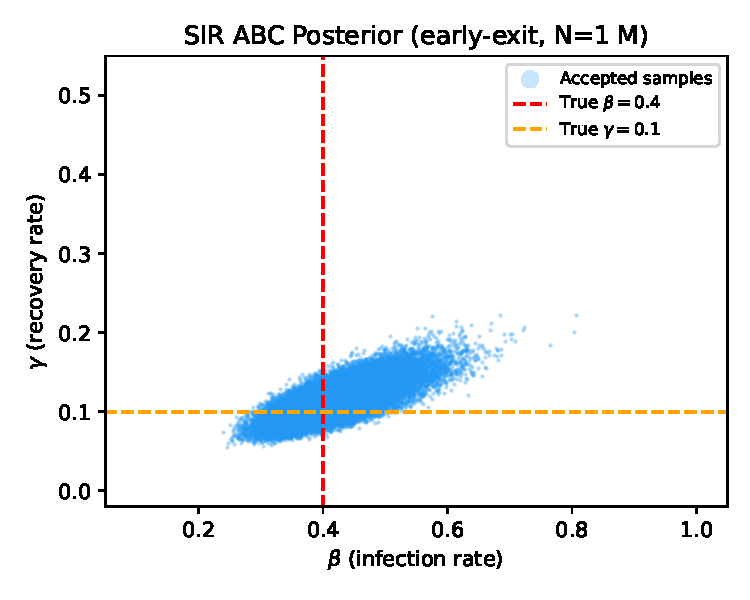
\includegraphics[width=0.96\columnwidth]{../figures/sir_posterior.pdf}
\caption{SIR ABC posterior samples in $(\beta, \gamma)$ space ($N=10^6$, early-exit).}
\label{fig:sir_posterior}
\end{figure}

\section{Sequential Performance Results}

\subsection{Gaussian Model}

\begin{table}[H]
\caption{Gaussian model: sequential performance.}
\label{tab:gaussian_performance}
\centering
\resizebox{\columnwidth}{!}{%
\begin{tabular}{rrrrr}
\toprule
Particles & Runtime (s) & Throughput (p/s) & Accepted & Acc.\ rate \\
\midrule
$10^4$ & $7.40 \times 10^{-4}$ & $13.5 \times 10^6$ & $443$ & $4.43\%$ \\
$10^5$ & $5.35 \times 10^{-3}$ & $18.7 \times 10^6$ & $4{,}390$ & $4.39\%$ \\
$10^6$ & $5.19 \times 10^{-2}$ & $19.3 \times 10^6$ & $43{,}907$ & $4.39\%$ \\
\bottomrule
\end{tabular}
}
\end{table}

\subsection{SIR Model}

\begin{table}[H]
\caption{SIR model: sequential performance (early-exit mode).}
\label{tab:sir_early_performance}
\centering
\resizebox{\columnwidth}{!}{%
\begin{tabular}{rrrrr}
\toprule
Particles & Runtime (s) & Throughput (p/s) & Accepted & Acc.\ rate \\
\midrule
$10^4$ & $0.206$ & $4.85 \times 10^4$ & $225$ & $2.25\%$ \\
$10^5$ & $2.12$ & $4.72 \times 10^4$ & $2{,}200$ & $2.20\%$ \\
$10^6$ & $21.15$ & $4.73 \times 10^4$ & $22{,}033$ & $2.20\%$ \\
\bottomrule
\end{tabular}
}
\end{table}

\begin{table}[H]
\caption{SIR model: sequential performance (fixed-$T$ mode).}
\label{tab:sir_fixed_performance}
\centering
\resizebox{\columnwidth}{!}{%
\begin{tabular}{rrrrr}
\toprule
Particles & Runtime (s) & Throughput (p/s) & Accepted & Acc.\ rate \\
\midrule
$10^4$ & $0.215$ & $4.65 \times 10^4$ & $225$ & $2.25\%$ \\
$10^5$ & $2.15$ & $4.65 \times 10^4$ & $2{,}200$ & $2.20\%$ \\
$10^6$ & $21.38$ & $4.68 \times 10^4$ & $22{,}033$ & $2.20\%$ \\
\bottomrule
\end{tabular}
}
\end{table}

\subsection{SIR Work Metrics}

\begin{table}[H]
\caption{SIR simulation steps per particle ($N = 10^6$).}
\label{tab:sir_steps}
\centering
\begin{tabular}{lcc}
\toprule
Mode & Mean steps & Std.\ dev. \\
\midrule
Early-exit & $64.2$ & $44.9$ \\
Fixed-$T$ & $160$ & $0$ \\
\bottomrule
\end{tabular}
\end{table}

\begin{figure}[H]
\centering
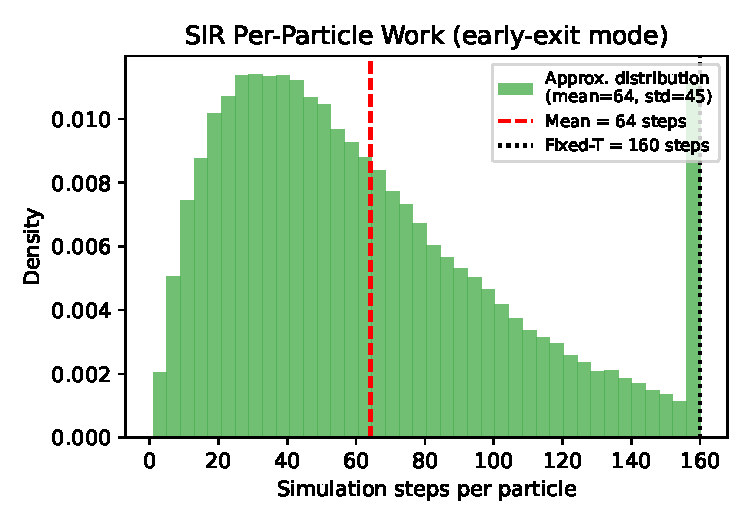
\includegraphics[width=0.96\columnwidth]{../figures/sir_step_histogram.pdf}
\caption{Distribution of SIR simulation steps per particle (early-exit mode, $N=10^6$).}
\label{fig:sir_steps}
\end{figure}

Early exit has std $44.9$ on steps. A warp on the GPU would wait on the
longest trajectory in the group.

\subsection{Workload Comparison}

\begin{table}[H]
\caption{Per-particle cost comparison ($N = 10^6$).}
\label{tab:workload_comparison}
\centering
\begin{tabular}{lrrr}
\toprule
Metric & Gaussian & SIR (early) & SIR (fixed) \\
\midrule
Runtime (s) & $5.19 \times 10^{-2}$ & $21.15$ & $21.38$ \\
Throughput (p/s) & $19.3 \times 10^6$ & $4.73 \times 10^4$ & $4.68 \times 10^4$ \\
Updates/s & --- & $64.2 \times 4.73 \times 10^4$ & $160 \times 4.68 \times 10^4$ \\
\bottomrule
\end{tabular}
\end{table}

\begin{figure}[H]
\centering
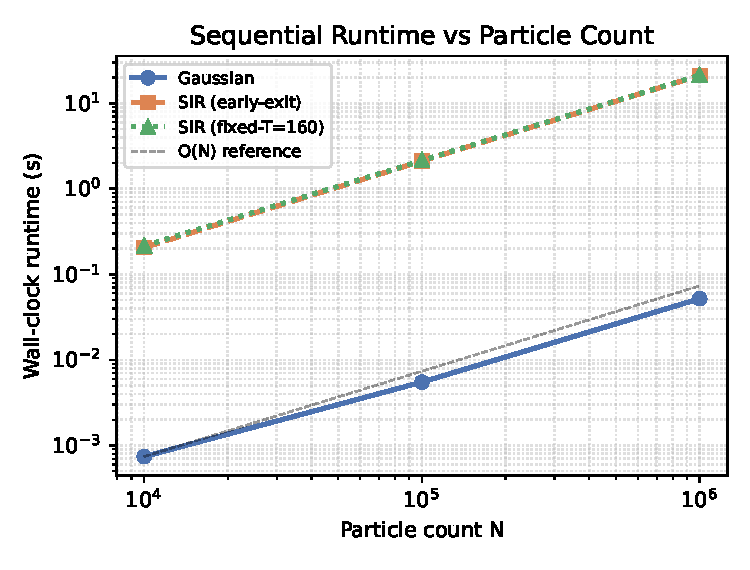
\includegraphics[width=0.96\columnwidth]{../figures/runtime_comparison.pdf}
\caption{Sequential runtime vs.\ particle count across all workloads (log--log scale).}
\label{fig:runtime_comparison}
\end{figure}

\section{Conclusion and Future Work}

The sequential sampler is in C++. Gaussian ABC at $\varepsilon=0.1$ has mean
and variance $0.501$ against $0.5$. SIR at $N=10^6$ takes about $21$\,s, versus
$0.05$\,s for Gaussian. Early exit averages $64$ steps (std $45$); fixed $T$ is
always $160$. $s_{\mathrm{obs}}$, $\sigma_k$, and $\varepsilon$ are in
\texttt{results/} and stay as they are.

Next we implement one particle per CUDA thread with the same models and
thresholds. Posterior mean/variance and acceptance rate are the check against
this CPU run. Profiling can wait until that kernel exists.

\bibliographystyle{IEEEtran}
\bibliography{references}

\end{document}
